% Options for packages loaded elsewhere
\PassOptionsToPackage{unicode}{hyperref}
\PassOptionsToPackage{hyphens}{url}
%
\documentclass[
]{article}
\usepackage{amsmath,amssymb}
\usepackage{lmodern}
\usepackage{iftex}
\ifPDFTeX
  \usepackage[T1]{fontenc}
  \usepackage[utf8]{inputenc}
  \usepackage{textcomp} % provide euro and other symbols
\else % if luatex or xetex
  \usepackage{unicode-math}
  \defaultfontfeatures{Scale=MatchLowercase}
  \defaultfontfeatures[\rmfamily]{Ligatures=TeX,Scale=1}
\fi
% Use upquote if available, for straight quotes in verbatim environments
\IfFileExists{upquote.sty}{\usepackage{upquote}}{}
\IfFileExists{microtype.sty}{% use microtype if available
  \usepackage[]{microtype}
  \UseMicrotypeSet[protrusion]{basicmath} % disable protrusion for tt fonts
}{}
\makeatletter
\@ifundefined{KOMAClassName}{% if non-KOMA class
  \IfFileExists{parskip.sty}{%
    \usepackage{parskip}
  }{% else
    \setlength{\parindent}{0pt}
    \setlength{\parskip}{6pt plus 2pt minus 1pt}}
}{% if KOMA class
  \KOMAoptions{parskip=half}}
\makeatother
\usepackage{xcolor}
\usepackage{longtable,booktabs,array}
\usepackage{calc} % for calculating minipage widths
% Correct order of tables after \paragraph or \subparagraph
\usepackage{etoolbox}
\makeatletter
\patchcmd\longtable{\par}{\if@noskipsec\mbox{}\fi\par}{}{}
\makeatother
% Allow footnotes in longtable head/foot
\IfFileExists{footnotehyper.sty}{\usepackage{footnotehyper}}{\usepackage{footnote}}
\makesavenoteenv{longtable}
\usepackage{graphicx}
\makeatletter
\def\maxwidth{\ifdim\Gin@nat@width>\linewidth\linewidth\else\Gin@nat@width\fi}
\def\maxheight{\ifdim\Gin@nat@height>\textheight\textheight\else\Gin@nat@height\fi}
\makeatother
% Scale images if necessary, so that they will not overflow the page
% margins by default, and it is still possible to overwrite the defaults
% using explicit options in \includegraphics[width, height, ...]{}
\setkeys{Gin}{width=\maxwidth,height=\maxheight,keepaspectratio}
% Set default figure placement to htbp
\makeatletter
\def\fps@figure{htbp}
\makeatother
\setlength{\emergencystretch}{3em} % prevent overfull lines
\providecommand{\tightlist}{%
  \setlength{\itemsep}{0pt}\setlength{\parskip}{0pt}}
\setcounter{secnumdepth}{-\maxdimen} % remove section numbering
\ifLuaTeX
  \usepackage{selnolig}  % disable illegal ligatures
\fi
\IfFileExists{bookmark.sty}{\usepackage{bookmark}}{\usepackage{hyperref}}
\IfFileExists{xurl.sty}{\usepackage{xurl}}{} % add URL line breaks if available
\urlstyle{same} % disable monospaced font for URLs
\hypersetup{
  hidelinks,
  pdfcreator={LaTeX via pandoc}}

\author{}
\date{}

\begin{document}

\hypertarget{vision}{%
\section{Vision}\label{vision}}

In questo documento viene descritta una linea generale dell'idea di
svolgimento del progetto.

\hypertarget{obiettivi}{%
\section{Obiettivi}\label{obiettivi}}

L'obiettivo è sviluppare un sitema con componenti \textbf{web
responsive} in grado di monitorare e di eseguire le azioni sotto
menzionate sul sistema di illuminazione pubblico di una città.

\hypertarget{assunti-preventivi}{%
\subsection{Assunti preventivi}\label{assunti-preventivi}}

\begin{itemize}
\tightlist
\item
  il gestore è in possesso di uno smartphone (Android o iOS) e nelle
  condizioni di utilizzare un browser web.
\end{itemize}

\hypertarget{obiettivi-obbligatori}{%
\subsection{Obiettivi obbligatori}\label{obiettivi-obbligatori}}

\begin{itemize}
\item
  \textbf{Rilevamento della presenza di persone} in prossimità della
  fonte luminosa: attraverso sensori eterogenei (bluetooth, IR,
  videocamere, ecc.) il sistema rileva la presenza di persone in un'area
  della città gestita dal sistema e attiva le luci di conseguenza.
\item
  Aumento/riduzione dell'intensità luminosa: il sistema deve essere in
  grado di comunicare attraverso un protocollo IoT l'aumento o la
  riduzione dell'intensità luminosa emessa da uno specifico impianto di
  illuminazione, permettendo una regolazione singola o per l'intera
  via/piazza (area coperta dal servizio).
\item
  Rilevamento automatico del guasto di un impianto di illuminazione: il
  sistema deve rilevare ogni eventuale malfunzionamento dell'impianto di
  illuminazione, notificando il gestore ed aprendo un ticket di
  assistenza su una piattaforma esterna che permetta di identificare la
  località del guasto.
\item
  Segnalazione manuale del guasto di un impianto di illuminazione: il
  sistema deve permettere di inserire manualmente un nuovo guasto ad un
  impianto di illuminazione.
\item
  Aumento/riduzione manuale dell'intensità luminosa: il sistema deve
  permette al gestore di aumentare/ridurre o riportare in modalità
  automatica l'illuminazione di un singolo impianto luminoso o di
  un'intera area coperta dal servizio.
\item
  Inserimento e gestione di un impianto luminoso: il sistema deve
  permettere al gestore l'inserimento di nuovi impianti luminosi e il
  loro inserimento o rimozione all'interno di un'area coperta dal
  servizio.
\item
  Aumento o riduzione globale dell'intensità luminosa: il sistema deve
  permettere al gestore l'aumento o la riduzione globale (su tutti gli
  impianti controllati dell'intensità luminosa, opzione particolarmente
  utile in condizioni di crepuscolo o luce lunare particolarmente
  intensa.
\end{itemize}

\hypertarget{obiettivi-secondari}{%
\subsection{Obiettivi secondari}\label{obiettivi-secondari}}

\begin{itemize}
\item
  modulare la luminosità a seconda della quantità di persone o tipologia
  di entità;
\item
  Rilevamento tipologia guasti (Guasti locali o distribuiti, guasti a
  sistemi di alimentazione);
\item
  Preset di illuminazione per le varie situazioni
\item
  integrazione con previsioni di eventi normali(alba e tramonto) ed
  anomali come eclissi;
\item
  Gestione multi utente (``gestore illuminazione pubblica'',
  ``installatore/manutentore'', ``Verificatore d'impianto'' , altro)
\item
  Pagina disponibile ai ``cittadini'' dove questi possano (seguendo 2/3
  passaggi, ad esempio caricando un'immagine del guasto) caricare una
  segnalazione di guasto.
\end{itemize}

\hypertarget{ottica-di-espansione-futura}{%
\subsection{Ottica di espansione
futura}\label{ottica-di-espansione-futura}}

\begin{itemize}
\item
  Integrazioni future con sistemi di alimentazione/UPS vari nella
  gestione guasti/distribuzione dell'alimentazione;
\item
  Api pubblica regolamentata utilizzabile in futuro da pannellistica a
  led per mostrare ai cittadini i risparmi o altro.
\end{itemize}

\hypertarget{vision-architetturale}{%
\section{Vision architetturale}\label{vision-architetturale}}

Visto l'\textbf{ambito critico} di operazione del prodotto software per
noi i capostipiti nello sviluppo di questo progetto saranno:
\textbf{alta modularità, alta scalabilità, alta resilienza e facile
estensibilità} dello stesso.

L'architettura seguirà quindi i principi base di un sistema a
microservizi che tenga conto di tutte queste importanti questioni.

\hypertarget{user-stories-casi-duso}{%
\subsection{User stories / casi d'uso}\label{user-stories-casi-duso}}

\begin{enumerate}
\def\labelenumi{\arabic{enumi}.}
\tightlist
\item
  login e logout di un operatore
\item
  collegamento di un impianto luminoso ai dati derivanti da un sensore
  (modalità automatica)
\item
  gestione manuale di un impianto luminoso
\item
  aumento o riduzione globale dell'intensità luminosa da parte di un
  operatore o tramite dati di un sensore
\item
  aumento o riduzione locale (per area illuminata) dell'intensità
  luminosa da parte di un operatore o tramite dati di un sensore
\item
  Gestione ticketing guasti
\item
  inserimento e gestione di un impianto luminoso
\item
  creazione, modifica e rimozione di nuove aree illuminate
\item
  tracciamento delle intensità luminose di ogni impianto.
\item
  Rilevamento della presenza in un'area illuminata e aumento automatico
  dell'intensità luminosa
\end{enumerate}

\hypertarget{utenti}{%
\subsection{Utenti}\label{utenti}}

Molteplici saranno gli utenti che utilizzeranno il sistema.

\begin{longtable}[]{@{}
  >{\raggedright\arraybackslash}p{(\columnwidth - 4\tabcolsep) * \real{0.3333}}
  >{\raggedright\arraybackslash}p{(\columnwidth - 4\tabcolsep) * \real{0.3333}}
  >{\raggedright\arraybackslash}p{(\columnwidth - 4\tabcolsep) * \real{0.3333}}@{}}
\toprule()
\begin{minipage}[b]{\linewidth}\raggedright
Utente
\end{minipage} & \begin{minipage}[b]{\linewidth}\raggedright
utilizzi
\end{minipage} & \begin{minipage}[b]{\linewidth}\raggedright
Tipo di requisito
\end{minipage} \\
\midrule()
\endhead
Semplice cittadino & Può vedere una dashboard relativa all'illuminazione
& Aggiuntivo \\
Gestore dell'illuminazione & Può impostare l'illuminazione &
Obbligatorio \\
Installatore/manutentore & Aggiunge nuove sezioni illuminanti, risolve i
guasti & Obbligatorio \\
\bottomrule()
\end{longtable}

\hypertarget{servizi}{%
\subsection{Servizi}\label{servizi}}

\begin{longtable}[]{@{}
  >{\raggedright\arraybackslash}p{(\columnwidth - 4\tabcolsep) * \real{0.3333}}
  >{\raggedright\arraybackslash}p{(\columnwidth - 4\tabcolsep) * \real{0.3333}}
  >{\raggedright\arraybackslash}p{(\columnwidth - 4\tabcolsep) * \real{0.3333}}@{}}
\toprule()
\begin{minipage}[b]{\linewidth}\raggedright
Servizio
\end{minipage} & \begin{minipage}[b]{\linewidth}\raggedright
Scopo
\end{minipage} & \begin{minipage}[b]{\linewidth}\raggedright
Tecnologia
\end{minipage} \\
\midrule()
\endhead
Mqtt & Comunicazione delle componenti IoT & Mosquitto \\
Database & Stoccaggio a lungo termine dei dati per un'analisi futura
degli stessi per prevenire guasti o risolvere situazioni ricorrenti &
Postgres \\
Coordinatore & Coordinamento e gestione diretta degli apparati
illuminanti & Python, Java, da vedere \\
ApiREST del sistema d'illuminazione & Api Backend per la webapp e altri
utilizzi futuri & Python, Flask \\
Backend/Api Ticketing & Gestisce il sistema di ticketing dei guasti &
Python, Flask \\
WebApp & Consente agli utenti(Definiti più avanti) di interfacciarsi con
il sistema & VueJs o React \\
\bottomrule()
\end{longtable}

\begin{figure}
\centering
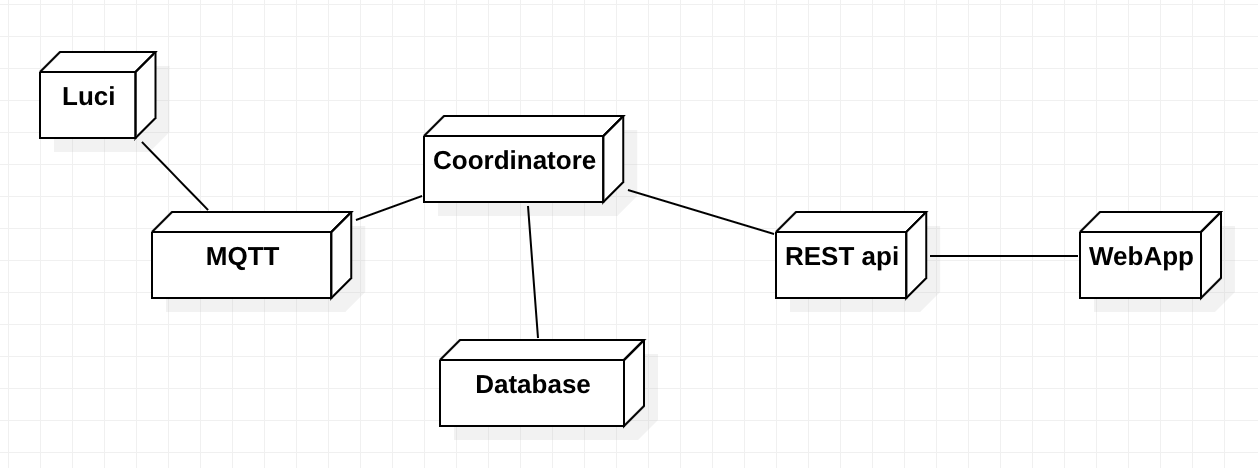
\includegraphics{grafico-servizi.png}
\caption{grafico-dei-servizi}
\end{figure}

\hypertarget{gestione-di-deploy}{%
\subsection{Gestione di Deploy}\label{gestione-di-deploy}}

Per il deploy sarà utilizzato \textbf{Docker} per consentire, alla
bisogna, lo scalare orizzontale del sistema, così da poter gestire più
utenti abbattendo i costi.

Il sistema sarà \emph{multi-tennant} as a service oppure installabile
\emph{on premise}.

\hypertarget{testing}{%
\section{Testing}\label{testing}}

Ognuno dei servizi avrà la sua specifica strategia di testing.

I test di ognuno dovranno avere comunque almeno l'80\% di code coverage
e dovranno essere correlati di report relativamente all'esecuzione degli
stessi.

\end{document}
